\clearpage

\section{Hardware}
\label{sec:hardware}

\subsection{Raspberry PI}
The Raspberry PI is a small computer in the form of a single board with a system on a chip. The SoC is a BCM2835 licensed from Broadcom. It has an ARM11v6 CPU running at 700 MHz with 256 (model A) or 512 MB (model B) SDRAM shared with the on board GPU. 

The unit was intended for educational use as a tool for promoting computer science in schools in the UK. It has instead largely been adopted by higher education, research and home users, although it still has a place in children schools.

\begin{figure}[h]
    \centering
    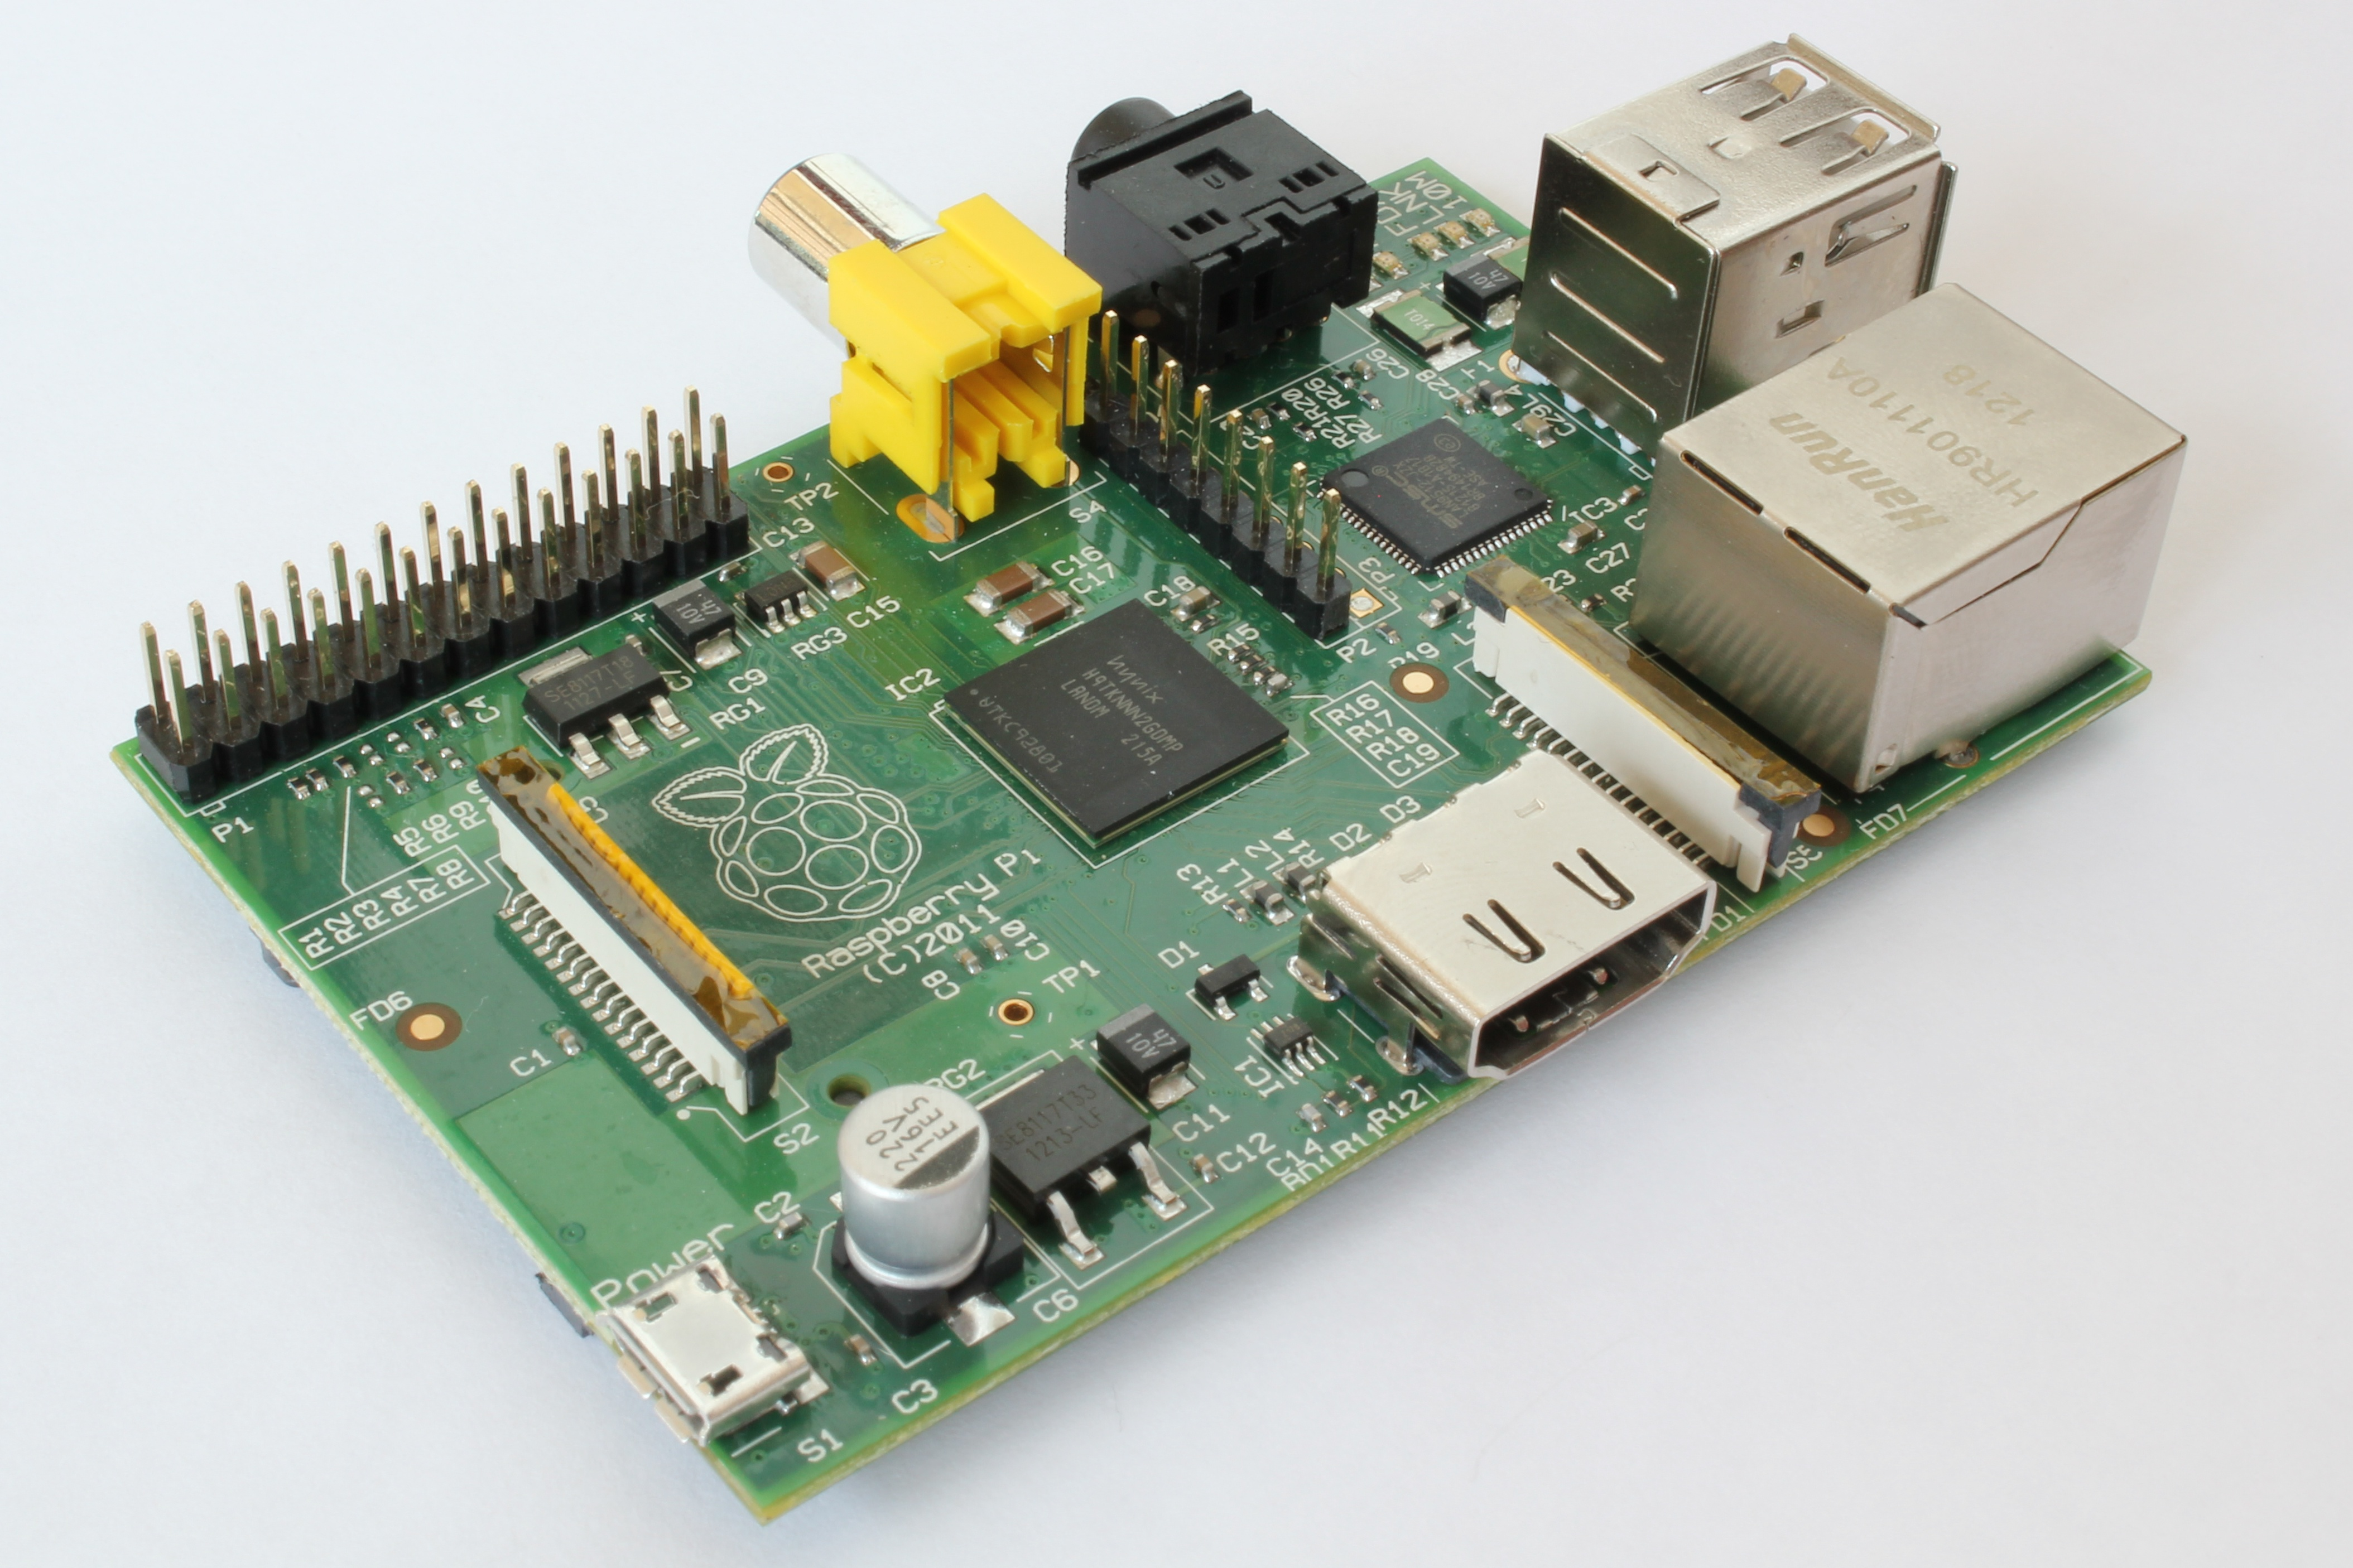
\includegraphics[width=0.8\textwidth]{hardware/RaspberryPi}
    \caption{A Raspberry PI}
    \label{fig:raspberrypi_hw}
\end{figure}

One of our concerns when we were researching this project, was the connection to the Ethernet, see the block diagram in Figure \ref{fig:pi_blockdiagram}.
It shows that the Ethernet adapter is a USB device connected to the onboard 3-port USB hub. This is only included on the model B version of the board. 
The model A only has a single USB port and does not include an Ethernet adapter, making the model B our only realistic choice.

A USB powered Ethernet implies a few things for the board. First, the computer has to poll the network adapter for data. 
Spending CPU time on polling the adapter with such an already weak device is something we would have liked to avoid, but could not. Secondly it also possibly means a higher power drain on both the CPU because of polling and the inclusion of a USB device itself.
It is however convenient that the USB device will use the same voltage as the board itself, and will not require any deregulation. 

\begin{figure}
	\centering
    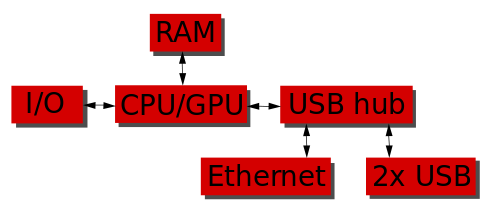
\includegraphics[width=0.5\textwidth]{hardware/raspberrypi_block_function}
    \caption{Layout of the functional blocks on the PI}
    \label{fig:pi_blockdiagram}
\end{figure}

\subsection{Configuration}
The PI comes with a number of different options for configuration. The board supports overclocking. Also, the amount of memory split with the shared memory GPU can also be manually set at boot using {\tt /boot/config.txt}.
Most unofficial documentation states that the PI requires a minimum of 16MB of RAM, but we were unable to get the PI to boot with less than 48 MB. 
With less than 48 MB, it seems the system never gets to boot.
The setting on our running hardware is therefore {\tt gpu\_mem\_512=48}.

The Raspberry also allows for easy overclocking without voiding the warranty, however reports suggest a real risk for data corruption on the SD card. There have also been reports of other kinds of instability, although it still works most of the time. The individual boards also display different degrees of tolerance to the overclocking, some working well at higher voltages and as much as double the memory speed, while others fail very easily.
The overclocking would also lead to increased power consumption and temperatures. In our tightly packed rig, this is a source of concern, but we will try it out none the less.

We do not want to deal with potentially unstable systems vulnerable to data corruption and undefined behavior, so we will only be looking further into this kind of performance enhancing of the hardware in the final part.

\subsection{Network}
For network switching we use a standard D-Link DES-1008D 10/100 switch. We cut our own network cables using a standard wire cutting tool to size to simplify cable pulling, and also limit waste.

\subsection{Power adapter}
As a power source we use a modified LaCie power supply. We chose this one because it is able to provide 5V up to 4.2A which should be enough to power our cluster of 8 devices.

\subsection{Alternative hardware}
The market for low power SoC computers is currently good, and units are selling faster\cite{growing_market}.
There are also new products from different manufacturers being launched continuously, and we will here take a closer look at a few of the current alternatives to the Raspberry PI.

\subsubsection{BeagleBone Black}
The BeagleBone Black is another open source low power mini computer on a single board. It is made by Texas Instruments and sold under the Creative Commons license.

The board is made from an AM3359 system on chip from Texas Instruments, sporting an ARMv7 Cortex-A8 running at 1 GHz with 512MB of DDR3 RAM. This board has a slightly weaker GPU than the PI. This is interesting as we will not be using the GPU anyway, and could help giving more power to the CPU.
We did not know about the release of this board when we did the planning for this project, but with it's very similar pricing (\$45 compared to \$35 as of this writing) and significantly more powerful CPU, it would make for an interesting comparison and alternative. The reported power consumption is riddled with uncertainty, but reports seem to place it slightly higher to that of the PI at 200-400mA compared to 300mA.

The improved instruction set architecture is also alluring, with this board providing an ARMv7 CPU, instead of the quite ancient ARMv6 on the PI.

\subsubsection{MK802}
Another board computer that is built as a USB stick by Chinese manufacturer Rikomagic.
It is based on a AllWinner A1X SoC running an ARMv7 Cortex-A8 at 1GHz and 1GB RAM. It's main purpose is as an Android test platform, but it also runs some Linux distributions, e.g. Ubuntu.
We were unable to find any official specs, but users report at least 1A is required to reliably run the 5V USB device. 
While the device is a lot more powerful than our alternatives, the added power drain would be difficult to accommodate on a larger scale, leaving it as a less interesting alternative.

\subsection{Cluster}
We currently have 8 devices in the cluster, with one acting as a load balancer. This leaves 7 worker nodes for answering queries.

\subsection{Power}
Our power supply is a 5V AC-DC converter with a maximum output of 4.2A at 5V. The expected maximum drain of the PI is listed at 700mA\cite{raspi_power_drain}. This would allow us to run at least $\frac{4.2A}{0.7A}=6$ PIs.
However we are not using the GPU or any other media related devices so we would expect this number to be somewhat lower, even under load.
